\section*{Discussion}
\label{sec:discussion}

\subsection*{\revise{Nonnegative sparse coding (NSC) in the brain}}
\mikeNote{I tried to make the Discussion flow better so that it reads less like a mingle-mangle of unrelated topics (while still incorporating all the reviewer rants). There's 2 topics here: 1) details/criticism of NSC as a model, 2) the concern that NSC might not apply to your favorite brain area. Feel free to move around or let me know if you approve.}
\revise{We reviewed compelling evidence that a wide range of neuronal responses 
can be understood as an emergent property of efficient population coding 
due to dimensionality reduction and sparsity constraints.
In particular, \ac{NSC} might be employed 
by sensory areas to efficiently encode external stimulus spaces,
by associative areas to conjunctively represent multiple behaviorally
relevant variables,
and by the basal ganglia to coordinate movement.}

\revise{\ac{NSC} is tightly connected to a number of unsupervised learning techniques,
such as \ac{NMF}
(a popular tool for high-dimensional data analysis \cite{Gillis2014}),
$k$-means clustering
(an algorithm used to partition $n$ observations into $k$ clusters \cite{Ding2005}),
and \textbf{\ac{ICA}}
(a computational method for separating a multivariate signal
into additive, statistically independent subcomponents).}
\revise{Both \ac{NMF} and \ac{ICA} are capable of decomposing high-dimensional data
into parts-based representations---in contrast to \ac{PCA}, which usually results in holistic representations \cite{LeeSeung1999}.}
As originally noted by Hoyer \cite{Hoyer2002},
if the fixed-norm constraint is placed on the rows of
\textbf{H} instead of the columns of \textbf{W},
Eq.~\ref{eqn:nsc-cost-function} can be directly interpreted as the joint
log-posterior of the basis functions and hidden components
in the noisy \ac{ICA} model \cite{HoyerHyvarinen2002}.
% In order for this connection to hold,
% the \ac{ICA} basis functions must be chosen to be nonnegative,
% and the independent components must have 
% exponential distributions \cite{Hoyer2002}.



Similarly, \ac{NSC} is closely related to compressed sensing
(for a recent review see \cite{GanguliSompolinsky2012}),
and a recent study has even suggested to combine the two
\cite{WangLi2010}.
Compressed sensing posits that neurons might implement 
dimensionality reduction by randomly projecting patterns of activity
into a lower-dimensional space,
namely by synaptically mapping $N$ upstream neurons to a downstream region
containing $M < N$ neurons. 
The theory of compressed sensing then provides the mathematical tools
to reconstruct the original space from the random projections.

\ac{NSC}, \ac{ICA}, and compressed sensing often make similar predictions
that only slightly differ in the nature of the basis function representation
necessary to achieve optimal reconstruction
(for details please refer to the Discussion of \cite{GanguliSompolinsky2012}).
For example, whereas \ac{ICA} emphasizes the statistical independence 
of unmixed sources
and compressed sensing requires basis function to be `maximally incoherent'
\cite{GanguliSompolinsky2012},
\ac{NSC} does not make any such assumptions
as long as the basis functions are nonnegative.


\subsubsection*{Potential neural mechanisms}

As a special case of efficient coding,
\ac{NSC} possesses metabolic advantages by employing
sparse population codes.
To operate efficiently, it has been suggested that the brain might enforce 
geometrical and biophysical constraints on axonal wiring 
\cite{LaughlinSejnowski2003}.
In addition to reducing overall wiring length
\cite{Cherniak1994}, the brain might also aim to minimize local delays
by favoring a high degree of local connectivity
\cite{Chklovskii2002}.
\revise{If connectivity reflects} coding \cite{Clopath2010},
it would not be surprising to find that such ecological considerations
carry over into brain function,
favoring sparse population codes and neuronal representations that are
local in functional space (i.e., parts-based).
However, wiring cost is likely to be only one of many constraints 
on the brain connectome, perhaps supplementing competitive pressures
for hub-mediated information exchange between network modules
\cite{Rubinov2015}.

In addition, evidence suggests that Hebbian-like synaptic plasticity rules
allow neurons to perform statistical inference on their inputs
\cite{Nessler2009,Carlson2013,MorenoBoteDrugowitsch2015,Oja1982}.
One particular study demonstrated through a mathematical proof
that a certain form of \textbf{\ac{STDP}} in combination with 
homeostatic synaptic scaling (i.e., \ac{STDPH})
can approximate the \ac{NMF} algorithm
\cite{Carlson2013}.
Similar to Oja's rule \cite{Oja1982}, which was developed to stabilize 
rate-based Hebbian learning
(effectively resulting in principal component analysis),
Carlson and colleagues showed that synaptic scaling acts as a 
homeostatic mechanism to stabilize \ac{STDP}
(effectively resulting in \ac{NMF}).
Interestingly, we were able to apply these ideas to 
electrophysiologically recorded neuronal activity observed in the \ac{RSC}
of rats during a spatial navigation task (Fig.~\ref{fig:NMF|RSC}; for experimental details see Supplementary Material). Both \ac{STDPH} and \ac{NMF} were able to recover key  features such as encoding spatial reference frames (i.e., allocentric and route-centric firing patterns) and position discrimination by reducing the dimensionality of behavioral variables (e.g., velocity, head direction, position).
The neuronal and population responses from NMF and STDPH were comparable to the experimental findings \cite{AlexanderNitz2015}.
Furthermore, the \ac{STDPH} model contained a highly flexible and generalizable code
that could automatically encode new routes through the same environment
without retraining \cite{Rounds2018}.

However, more research is needed to elucidate any potential connection 
between \ac{NSC} and the many different synaptic plasticity rules 
commonly found across brain regions,
different stages in the life of an animal, and animal species
(e.g., \cite{Froemke2010,BCM1982}).

\begin{figure}[ht!]
	\centering
	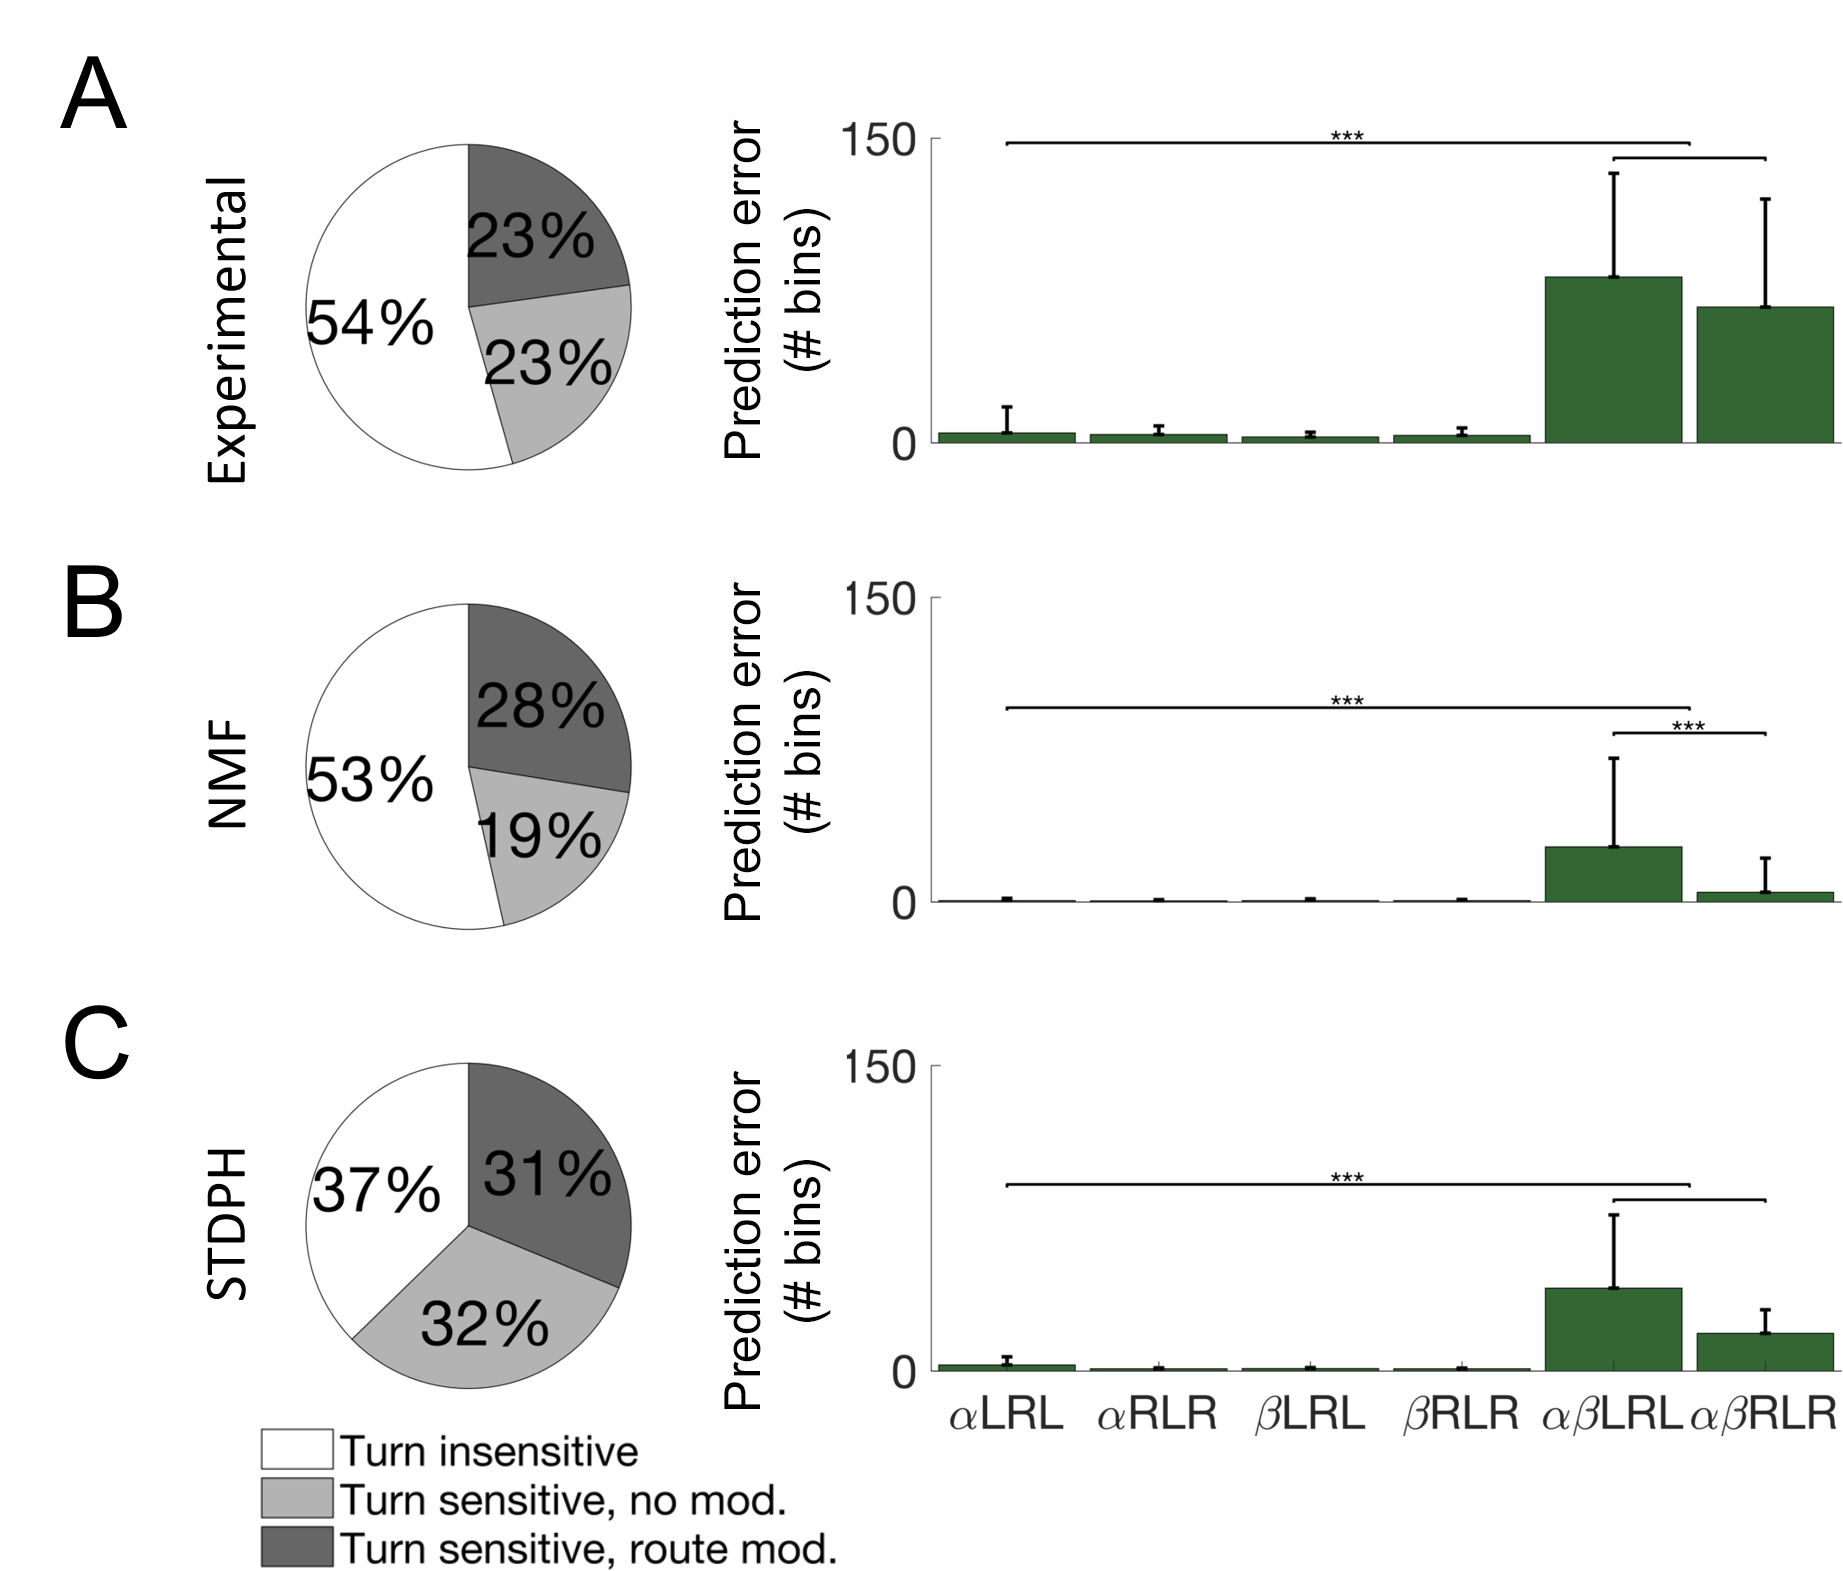
\includegraphics[width=0.95\textwidth]{fig-rev2-rsc}
    \caption{
    	Comparison between experimental data and two 
        computational models of rat \ac{RSC} suggest a functional 
        similarity between \ac{STDPH} and \ac{NMF}.
        \revise{Rats used two turn sequences 
        (inbound: left-right-left, LRL; outbound: right-left-right, RLR)
        to traverse a W-shaped track located at two different allocentric locations
        ($\alpha$, $\beta$).}
        \textbf{\emph{A}},
    		Experimental data from \cite{AlexanderNitz2015}.
        \textbf{\emph{B}},
            Simulated using NMF with sparsity constraints.
        \textbf{\emph{C}},
            Simulated by evolving \ac{STDPH} parameters 
            to fit experimental data \cite{BeyelerCarlsonChou2015,Carlson2014}.
        \revise{\emph{Left column}: Functional neuron type distributions.
        \emph{Right column}: Movement prediction errors (arbitrary units)
        based on correlation matrices from population responses
        \cite{AlexanderNitz2015,Rounds2018}.
        Prediction error between even and odd trials
        for the same position and route (prefix $\alpha$ or $\beta$) 
        was much smaller than across tracks (prefix $\alpha\beta$;
        Kruskal-Wallis and Tukey's range test, ***$= p < 0.001$).
        For details see Supplemental Material.}
	}
 	\label{fig:NMF|RSC}
\end{figure}
            
%         (adapted \revise{with permission} from \cite{Rounds2018}). 
%         Using methods described in \cite{AlexanderNitz2015}, 
%         we compared functional neuron type distributions (left column)
%         and average \revise{movement} prediction errors (right column)
%         observed \emph{in vitro} (\textbf{\emph{A}}) with those
%         produced by each model (\textbf{\emph{B, C}}).
%         Average error corresponded to correlation matrices 
%         representing reconstructed position within a route. 
%         For details, see Supplementary Materials.
%         Separate \revise{allocentric} positions of the W-shaped track are represented 
%         by the symbols $\alpha$ and $\beta$. 
% %         Outbound and inbound runs were made up of 
% %         opposite turn sequences (left-right-left (LRL) 
% %         and right-left-right (RLR), respectively.
%         Reconstructions between \revise{trials occurring on the same track position are represented by that position (e.g., $\alpha$ or $\beta$), and are low since the neural activity represents the same movements and positions. Alternately, reconstructions of position between the (two \revise{different} track positions, which could also occupy different orientations,} are represented by
%         $\alpha \beta$. \revise{Reconstruction errors in this case are high since neural activity representing dissimilar actions and locations are compared.}




\subsubsection*{Model limitations}

Although \ac{NSC} has proved useful in understanding
a variety of neuronal responses
as an emergent property of efficient population
coding based on dimensionality reduction and sparse coding,
there are some limitations to this theory.

\revise{First, there is increasing evidence that several motor variables are encoded
throughout the brain, including early sensory areas 
\cite{CrochetPetersen2006,Pachitariu2015,Musall2018,Stringer2018}.
For example in the mouse, running modulates the gain of visual inputs 
\cite{Mineault2016,NiellStryker2010} 
and is critical for integration of visual motion \cite{Ayaz2013,Saleem2013}.
A potential explanation for these widespread effects is that 
certain movements reflect changes in the animal's internal state,
such as increased arousal during running \cite{NiellStryker2010}.
Another study found that stimuli and behavior 
were represented together in mouse \ac{V1} as a
mixed representation: there were not separate sets of neurons
encoding stimuli and behavioral variables, but each
neuron multiplexed a unique combination of sensory and
behavioral information \cite{Stringer2018}.
Interestingly, these results were not specific to visual cortex, but were seen across
wide regions of the mouse forebrain,
suggesting that neuronal activity in these areas is more than just an efficient
encoding of sensory stimuli.}

Second, a practical limitation of dimensionality analyses in general
is that the apparent dimensionality of the population response changes
systematically with the complexity of the input \revise{space}
\cite{SpanneJorntell2015,Cowley2016,Mazzucato2016}.
For practical purposes, simulated models of neuronal circuitry are typically
built with far fewer units than the number of neurons in the real network.
By excluding input dimensions that are present in the brain,
one will implicitly guide the simulated model away from spurious interactions
that the real circuitry would have to handle.
As a result, the simulated model might underestimate 
the true complexity of the task.

Third, \revise{a similar argument can be made for the apparent sparsity of neuronal responses
in a variety of brain regions, which might be due to researchers typically presenting 
small sets of stimuli.
Indeed, one study that applied \ac{PCA} to monkey \ac{V1} 
showed that one needs to look at many principal components to decode natural images,
and that these principal components reflect contributions 
from most of the recorded neurons \cite{Cowley2017}.
Similar results have been reported for a large number of stimuli and neurons
in mice \cite{Stringer2018}.}

\revise{Part of the confusion about the role of sparse coding in the brain
may arise} from the wide variety of definitions of sparsity
used in the literature:
In its widest possible theoretical sense,
a neuron population exhibits sparse activity if the average activation ratio
remains below 50\% for binary neurons 
or below 100\% for thresholded,
rate-based neurons \cite{SpanneJorntell2015}.
However, it is not surprising that different brain areas might employ
different degrees of sparsity.
\revise{For example, a network of `grandmother' cells might be able to implement
a maximally sparse code, but it would have to do so by sacrificing representational
capacity (as in Fig.~\ref{fig:sparse-parts}) and fault tolerance
(i.e., the capacity to handle neuronal noise or the loss of a subset of neurons)
\cite{Foldiak1990,SpanneJorntell2015}.
Instead, some brain areas might prefer to operate at a degree of sparsity that
still allows for some level of robustness or adaptability.
It is conceivable that this `point of operation' might depend on the complexity
of the stimulus to be encoded or the task to be performed---for example,}
favoring an extremely sparse code in \ac{V1}
\cite{OlshausenField1996},
but giving rise to a slightly denser code with 
greater representational capacity in higher-order visual areas
such as \ac{MSTd}, 
which could lead to compact and multifaceted encodings
of various perceptual variables
(see Discussion in \cite{Beyeler2016}).



\subsection*{\revise{Future directions}}

In addition to the areas highlighted above, 
the essential components of \ac{NSC} might be present 
in other brain regions not traditionally associated 
with the efficient encoding of information.
We offer three testable predictions of this theory:

First, we suggest that a variety of neuronal response properties
can be understood as an emergent property of efficient population coding 
based on dimensionality reduction.
Depending on input stimulus and task complexity,
we expect the dimensionality of the population code to be adjusted
according to the bias-variance dilemma
(Fig.~\ref{fig:nsc-bias-variance-dilemma}).
This point of operation might differ across brain areas---for example,
favoring neurons that respond to a small number of stimulus dimensions
in \ac{V1} \cite{OlshausenField1996},
but giving rise to mixed selectivity in higher-order brain areas
such as \ac{MSTd} \cite{Beyeler2016} and
\ac{RSC} \cite{Rounds2016,Rounds2018}.

Second, we predict that parts-based representations can explain
\acp{RF} of neurons in a variety of \revise{sensory and associative cortices},
including but not limited to those brain areas discussed here. 
In agreement with the literature on basis function representations
\cite{PougetSejnowski1997,PougetSnyder2000,Poggio1990},
we expect parts-based representations
to be prevalent in regions where neurons
exhibit a range of tuning behaviors \cite{Beyeler2016},
display mixed selectivity \cite{Fusi2016,Eichenbaum2017},
or encode information in multiple reference frames 
\cite{AlexanderNitz2015,Rounds2016,Rounds2018}.

Third, where such representations occur, we expect the resulting
neuronal population activity to be relatively sparse,
in order to encode information both accurately and efficiently.
As noted above, sparse codes offer a trade-off between 
dense codes (where every neuron is involved in every context,
leading to great memory capacity but suffering from cross talk among neurons)
and local codes (where there is no interference, 
but also no capacity for generalization).


\subsubsection*{\revise{Evidence against NSC in prefrontal and motor cortices}}

\revise{Two prominent examples where \ac{NSC} might not apply
are \ac{PFC} and \ac{M1}.
For one, studies indicate that the population code in these regions
may be quite dense (as in Fig.~\ref{fig:sparse-parts}A).
For another, dimensionality reduction studies in these regions suggest that 
features are encoded by most neurons in the population, 
arguing against a sparse parts-based representation 
\cite{Gallego2017,churchland2007,CunninghamYu2014,Kobak2016,Mante2013}.}

\revise{In the \ac{PFC}, individual neurons typically encode 
multiple task-related signals at once, 
including the animal's upcoming choice, the context, 
and the strength of the sensory evidence \cite{Mante2013,Rigotti2013,Kobak2016}.
Consequently, many recent studies have adopted dimensionality reduction
to analyze these populations and to find features that are not apparent
at the level of individual neurons \cite{CunninghamYu2014}.}

\revise{Similarly, responses in \ac{M1} are neither sparse nor parts-based
\cite{Scott2008,Russo2018,Gallego2017,Shenoy2013}.
Although it is possible to subdivide \ac{M1} based on the distribution of
cortico-motoneuronal cells, the projections of \ac{M1} neurons to different upper limb muscles
are greatly intermingled \cite{RathelotStrick2009}, 
arguing against a parts-based representation.
In addition, it is possible to accurately decode the activity of many upper limb muscles
based on the activity from neurons located within a small area of \ac{M1}
\cite{Shenoy2013}.
Furthermore, \ac{M1} neurons tend to be active during most movements, 
which argues against a sparse activation.
This may be due to the role of the motor system, which is to cause behavior, 
rather than represent features.}

\revise{Whereas feedforward neural networks are better predictors 
of neuronal processing in early sensory areas, it is interesting to note that
motor activity seems to be well represented by recurrent neural networks \cite{Tanaka2016}.
In addition, compressed sensing might be a good theoretical framework for the motor system: 
When Trautmann and colleagues \cite{trautmann2017} applied random projection theory 
to data from three previous studies of \ac{M1},
they found that the reconstructed neural dynamics yielded results quite similar 
to those derived from spike sorting.}



\subsubsection*{\revise{Potential for NSC in the hippocampus}}

\revise{There are aspects of the hippocampus that are comparable to the ideas 
of \ac{NSC} proposed here.
For example, the dentate gyrus is often associated with sparse activity
\cite{GoodSmith2017,JungMcNaughton1993,SenzaiBuzsaki2017}.
The expansion from a dense, enthorhinal cortex coding to sparse dentate gyrus 
activity suggested a mechanism of pattern separation
\cite{Marr1971,TrevesRolls1994}.
Since these early theories, accumulating evidence has supported 
the role of the dentate gyrus in pattern separation 
\cite{GoodSmith2017,SenzaiBuzsaki2017,YassaStark2011}.
However, the dentate gyrus projects to a highly recurrent CA3 region, 
which does not appear to be sparse or reduce dimensionality. 
Rather, the CA3 region has a role in pattern completion through auto-association 
\cite{KnierimNeunuebel2016,Marr1971,TrevesRolls1994}.
Another feature of hippocampal processing that is related to \ac{NSC} 
may be the place cell itself.
Sparsity has long been used as a metric for place cell quality \cite{Skaggs1996}.
A place cell is said to be sparse if it fires in a small region of the environment, 
and this is related to how much spatial information that cell encodes. 
In a sense, each place cell can be thought of as a ``part'' of the environment 
and these parts cover the entire environment. 
Although this evidence points to sparse, parts-based, 
and reduced coding in some hippocampal regions, 
it does differ from the \ac{NSC} representations in sensory areas.
That is, sparse coding as defined above for sensory areas is not necessarily the same 
as sparsity or as sparse activity leading to pattern separation. 
Still, it would be of interest to apply \ac{NSC} to the hippocampal inputs, 
similar to the methods applied to \ac{RSC} 
during a spatial navigation task \cite{Rounds2018},
to see if sparse, reduced basis functions emerge in other regions.}


\subsubsection*{\revise{Potential for NSC in parietal cortex}}

Analogous to our modeling work in \ac{MSTd} \cite{Beyeler2016},
it might be possible to apply \ac{NSC} to other areas of the posterior parietal
cortex that are involved in multisensory heading perception.
Areas such as the \ac{VIP} and \ac{VPS} are also known to respond to optic flow,
but they increasingly respond to inertial vestibular stimulation as well
\cite{Chen2011}.
Although the degree of sparsity of the population code in \ac{VIP} and \ac{VPS} is not known,
the fact that neurons in these areas respond to mixtures of visual and vestibular
heading cues make them prime examples 
to be examined with an \ac{NSC} based modeling approach.

Elsewhere in parietal cortex, single neurons act as basis functions 
to represent the spatial configuration of objects 
with respect to multiple reference frames
(e.g., by transforming eye-centered to body-centered coordinates).
\cite{Poggio1990,PougetSejnowski1997,PougetSnyder2000}.
This is similar to the integration of multimodal heading cues mentioned above,
as well as to other associative areas such as \ac{RSC},
which demonstrates conjunctive coding of various spatial navigation cues
\cite{AlexanderNitz2015,Rounds2018}.
There is further evidence that actions are represented in parietal cortex
with respect to arbitrary and abstract reference frames, 
such as with respect to a planned route through an environment \cite{nitz2009parietal}.
From a theoretical standpoint, \ac{NSC} seems a good candidate to find an efficient,
reference-frame agnostic representation of various behaviorally relevant variables
\cite{LouieGlimcher2012,louie2015adaptive,andersen1997multimodal,BenHamed2003},
but future studies will have to address these issues step by step.


\section*{\revise{Conclusion}}

\revise{In conclusion, there is increasing evidence that \ac{NSC} can account for
neuronal response properties in a number of sensory and associative cortices
as well as the basal ganglia.
Although \ac{NSC} might not apply to \ac{PFC} and motor cortex,
the success of \ac{NSC} based models across brain regions 
warrants further investigation.}




